% This is samplepaper.tex, a sample chapter demonstrating the
% LLNCS macro package for Springer Computer Science proceedings;
% Version 2.20 of 2017/10/04
%
\documentclass[runningheads]{llncs}
%
\usepackage{pgfgantt}

\usepackage{graphicx}
\usepackage[strings]{underscore}
\usepackage[hyphens]{url}
\usepackage{ragged2e}
\usepackage{tabularx}

\setlength{\parindent}{0in}
% Used for displaying a sample figure. If possible, figure files should
% be included in EPS format.
%
% If you use the hyperref package, please uncomment the following line
% to display URLs in blue roman font according to Springer's eBook style:
% \renewcommand\UrlFont{\color{blue}\rmfamily}
\renewcommand\refname{Literaturangaben}

\begin{document}
%
\title{Hauptprojekt \\~\\ Konzeption und prototypische Implementierung einer verteilten Autoscaling-Architektur für Cloud-Bursting mit Container-as-a-Service}
%
\titlerunning{Hauptprojekt}
% If the paper title is too long for the running head, you can set
% an abbreviated paper title here
%
\author{Christian F. Bargmann}
%
% \authorrunning{F. Author et al.}
% First names are abbreviated in the running head.
% If there are more than two authors, 'et al.' is used.
%
\institute{Hamburg University of Applied Sciences, Berliner Tor 5, 20099 Hamburg, Germany \\
	\email{christian.bargmann@haw-hamburg.de} \\
	\url{https://www.haw-hamburg.de}}
%
\maketitle              % typeset the header of the contribution
%
\begin{abstract} Cloud-Bursting ist ein Betriebsmodell, bei dem eine Anwendung in einer privaten Cloudumgebung oder einem Rechenzentrum betrieben wird, jedoch automatisch Ressourcen einer öffentlichen Cloud provisioniert werden, wenn die Nachfrage nach Rechenkapazität ansteigt. Die Entscheidung, anhand welcher Kriterien Ressourcen in eine öffentliche Cloud ausgelagert werden, wie sich die provisonierten Ressourcen in die lokal betriebene Infrastruktur integrieren lassen und welches Servicemodell des Cloud-Providers verwendet werden soll, ist in den vergangenen Jahren in den Fokus aktueller Forschung gerückt. Dieses Hauptprojekt konzeptioniert, implementiert und evaluiert eine verteilte Autoscaling-Architektur für Cloud-Bursting in Hybrid-Clouds, die automatisiert Ress\-ourcen auf Basis von Metriken als Container-as-a-Service bei mehreren Cloud-Service-Providern provisionieren und skalieren kann.
		
	\keywords{Cloud Bursting \and Cloud Computing \and Autoscaling \and \newline Container \and Software Architecture}
\end{abstract}
%
%
%
	
\section{Einleitung} \label{motivation}
	
Cloud-Bursting ist ein Betriebsmodell, bei dem eine Anwendung in einer privaten Cloudumgebung oder einem Rechenzentrum betrieben wird, jedoch automatisch Ressourcen einer öffentlichen Cloud provisioniert werden, wenn die Nachfrage nach Rechenkapazität ansteigt. Bei diesem hybriden Betriebsmodell wird die eigene Infrastruktur vollständig genutzt, so dass eine Anzahl von Servern in eigener Verantwortung und Kontrolle betrieben werden kann. Gleichzeitig besteht bei Lastspitzen die Möglichkeit, die Anwendung ganz oder teilweise in eine externe, öffentliche Cloud zu verlagern. \\
	
Die wichtigste Technologie bei Cloud-Computing zum Hosten und Verwalten von Anwendungen ist die Virtualisierung. Traditionell wird Hardware-Level-Virtualisierung, auch bekannt als Hypervisor-basierte Virtualisierung, zur Verwaltung von virtuellen Maschinen (VMs) in Cloud-Rechenzentren verwendet. Ein grosser Fortschritt in der Virtualisierungstechnologie ist die Containerisierung von Anwendungen, die auch als Virtualisierung auf Betriebssystemebene bekannt ist. Aufgrund der besseren Portabilität, des geringen Ressourcenbedarfs und der einfachen Skalierbarkeit im Vergleich zur VM-basierten Virtualisierung, hat Containerisierung in den letzten Jahren deutlich Popularitaet gewonnen. Containerisierung eignet sich für die Verwaltung von Microservices, da sie das schnelle Starten und Beenden von Containern und somit schnelle Skalierbarkeit unterstützt, während die VM-basierte Virtualisierung vergleichsweise mehr Zeit für das Starten und Beenden der VM benötigt [6], [7]. Viele Cloud-Service-Provider (CSPs) bieten Container-as-a-Service Angebote an, mit denen sich Container in einer Cloud-Umgebung betreiben lassen, ohne darunterliegende Infrastruktur selbst verwalten zu muessen. \\

Was ist das Problem? \\
Bruecke zwischen mehreren Cloud-Plattformen, Integration in die eigene Infrastruktur, Provider-spezifische Interfaces \\

In dieser Arbeit wird eine verteilte Autoscaling-Architektur für Cloud-Bursting in Hybrid-Clouds vorgestellt, die automatisiert Ressourcen auf Basis von Metriken als Container-as-a-Service bei einem CSP provisionieren und skalieren kann. Die vorgestellte Architektur ist in der Lage, Anwendungen ueber mehrere Cloud-Umgebungen hinweg zu skalieren und provisionierte Ressourcen von mehreren Anbietern parallel in die eigene lokale Infrastruktur einzubinden. Fuer die automatische Skalierung von internen Ressourcen bei Lastspitzen zu CSPs werden Metriken aus externen Monitoring-Systemen genutzt, statt eigene Metriken zu implementieren. Im Gegensatz zu Anderen Ansaetzen (vgl. Abschnitt \ref{work}.) setzt die hier praesentierte Loesung nicht vorraus, das lokal ein Container-Cluster betrieben wird, was den Einsatz dieser Loesung attraktiv fuer Anwender macht, die kein Container-Cluster betreiben koennen, aber trotzdem ein Autoscaling fuer lokal betriebene Anwendungen haben moechten. Auch muessen lokal betriebene Anwendungen nicht modifiziert werden, um durch die vorgestellte Architektur skaliert zu werden. Die Komponenten der Autoscaling-Architektur koennen sowohl On-Premise, als auch extern bei einem CSP betrieben werden.

	
\section{Related Work} \label{work}
	
\subsection{Cloud-Bursting Architekturen}
	
Danayi et al. \cite{danayi_opencot_2019} präsentieren in ihrer Arbeit eine Implementierung eines Cloud Managers für das Internet of Things. Die vorgestellte Architektur nutzt Function-as-a-Service als Servicemodell, um bei Lastspitzen einzelne Funktionen zu einem öffentlichen Cloud-Provider auszulagern. Hierbei wird ein zentraler Cloud-Broker als Gateway-Komponente verwendet, der sämtliche Funktionsanfragen entgegennimmt und Logik zur Skalierung von Ressourcen an eine Controller-Komponente delegiert. Das Framework nutzt und speichert eigene Metriken für die Skalierung von Ressourcen und ist auf die Programmiersprache Python beschränkt. Für das Internet of Things bietet sich FaaS als ein geeignetes Servicemodell an, jedoch kann FaaS für viele Anwendungszenarien zu feingranular sein. \\
	
Biswas et al. \cite{biswas_auto-scaling_2015} erläutern eine Architektur für einen Cloud Broker, der sowohl proaktives, als auch reaktives Autoscaling für Anwendungen bei Lastspitzen realisiert. In einer fortführenden Arbeit werden Skalierungsmethoden anhand von Kostenanalysen präsentiert \cite{biswas_hybrid_2017}. Hierbei wird der Cloud Broker bei einem Drittunternehmen eingesetzt, welches im Bedarfsfall Ressourcen für die Private Cloud des Klienten bei einem Public-Cloud-Anbieter provisioniert. Der Klient hat keine Kontrolle über den eingesetzten Broker des Drittunternehmens, ebenso ist der Broker stark gekoppelt an die Schnittstellen des Public-Cloud-Providers. \\
	
Ye et al. \cite{ye_auto-scaling_2017} stellen eine Autoscaler-Architektur und prokative, sowie reaktive Skalierungsmethoden vor, die in einer containerbasierten, privaten Cloudumgebung eingesetzt werden können und sowohl das aktuelle Anfragevolumen, als auch Service Level Agreements (SLAs) für die geeignete Skalierung von Ressourcen berücksichtigen. Zwar werden hier automatisch Ressourcen bei Lastspitzen in der eigenen private Cloudumgebung skaliert, allerdings werden  keine externen Ressourcen hinzugezogen. \\
	
In einem Artikel stellt Chandra \cite{chandra_cloud_2020} eine Möglichkeit für Cloud-Bursting mithilfe der Kubernetes-Erweiterungen Virtual Kubelet\footnote{https://github.com/virtual-kubelet/virtual-kubelet} und KIP\footnote{https://github.com/elotl/kip} vor. Die vorgestellte Methode setzt den Betrieb eines eigenen Clusters in der privaten Cloudumgebung voraus und nutzt Autoscaling-Funktionalitäten des Container-Orchestrators Kubernetes für die horizontale Skalierung von Container-Instanzen. Es wird vorausgesetzt, dass die zu skalierenden Instanzen zuvor als ein Deployment im Cluster angelegt worden sind. Weiterhin beschreibt Mennig \cite{mennig_cloud_2020} einen Multicluster-Ansatz mit dem Einsatz von Service Meshes, um Cloud Bursting umzusetzen. Hier wird Cluster-as-a-Service als Servicemodell beim Public-Cloud-Provider genutzt, um Compute Cluster zu provisionieren und diese in die on-premise betriebene Cluster-Infrastruktur einzubinden. Ein Service-Mesh wird für die Cross-Cluster-Kommunikation von Ressourcen verwendet, gemeinsam mit einem Multicloud-Scheduler um Workloads bei Lastspitzen über mehrere Cluster zu verteilen. Auch hier wird jedoch der Betrieb einer eigenen Cloud-Infrastruktur vorausgesetzt, ebenso wird Expertenwissen benötigt für die Installation und Wartung der Cluster-Erweiterungen, was für viele Unternehmen ein nicht zu unterschätzender Aufwand ist.
	
\subsection{Provisionierung von Ressourcen}

Eine geeignete Skalierung von Ressourcen ist in verteilten Umgebungen wie Clouds wichtig. Eine Unterskalierung kann zu einer vollstaendigen Auslastung der Ressourcen führen, was im Fall von ARs zu hohen Antwortzeiten oder einer großen Anzahl abgelehnter Anfragen führt.  Eine Ueberskalierung wiederum, kann zu nicht ausgelasteten Ressourcen führen, sodass der Zusatzkosten für ungenutzte Rechenleistung entstehen. \\

Die Entscheidung über die Allokierung oder Freigabe von Cloud-Ressourcen basiert in der Regel auf einigen überwachten oder vorhergesagten Low-Level-Performance-Indikatoren (z. B. Auslastung von Ressourcen wie CPU, Speicher, Netzwerkbandbreite) oder High-Level-Indikatoren (z. B. Antwortzeit, Anfragerate). Weitere Metriken um ein Quality of Service (QoS) zu gewaehrleisten, werden auch in [17] und [18] vorgeschlagen. Zusammenfassend ist das Ziel dieser Arbeiten, genau dann automatische Skalierungsmechanismen auszulösen, um die Werte der ueberwachten Indikatoren innerhalb bestimmter Thresholds zu halten. Diesem Ansatz folgend, arbeitet die hier vorgestellte Autoscaling-Architektur mit Service-Level-Agreements (SLOs), um vom Application Manager festgelegte Werte fuer Indikatoren zu realisieren. \\

Eine automatische Skalierung von Ressourcen kann reaktiv durchgefuehrt werden, zum Beispiel als Folge von Änderungen der Arbeitslast, oder proaktiv, d. h. nach Vorhersagen von Änderungen der Arbeitslast. In mehreren Arbeiten werden auch Kombinationen der beiden Ansätze vorgeschlagen 19], [20], [21], [22], [23]. Desweiteren gibt es Arbeiten wie xxx, xxx und xxx, in denen maschinelles Lernen und analytische Verfahren fuer eine praediktive Autoskalierung vorgestellt werden. In dieser Arbeit wird eine reaktive Skalierungsstrategie praesentiert und in Abschnitt xx im Detail erlaeutert.
	
\section{Architekturübersicht}{Ziel der Projektarbeit}
	
Ziel dieses Hauptprojekt ist die prototypische Konzeption und Implementierung einer Architektur für Cloud-Bursting, die innerhalb einer Organisation arbeitet und automatisiert Ressourcen auf Basis von Metriken als Container-as-a-Service bei einem Public-Cloud-Anbieter provisioniert und skaliert. \\
	
Im Gegensatz zu Lösungen die auf Cloud-Infrastruktur aufsetzen, muss die zu skalierende Anwendung hierbei nicht auf einer eigenen Cloud-Infrastruktur betrieben werden. Hierdurch soll sich Cloud-Bursting auch für Anwendungen umsetzen lassen, die nicht für den Einsatz in Cloudumgebungen geeignet sind. Anders als Architekturen, die ohne den Einsatz von eigener Cloud-Infrastruktur auskommen, soll sich die Architektur in bestehende Monitoring-Lösungen wie z.B. Prometheus\footnote{https://prometheus.io} integrieren lassen und Metriken von externen Systemen für die geeignete Skalierung von Ressourcen heranziehen, statt eigene Metriken in Softwarekomponenten zu implementieren.
	
\subsection{Architektur}
	
\begin{figure}[h]
	\centering
	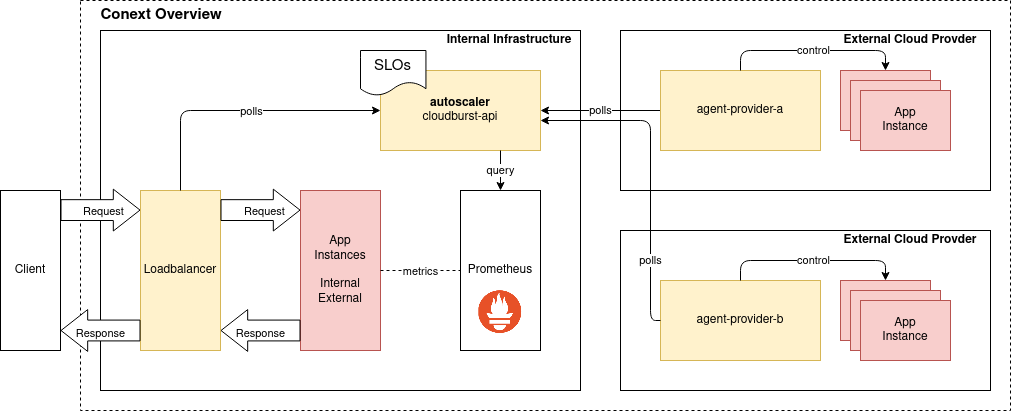
\includegraphics[width=1.0\linewidth,scale=1.0]{images/context.png}
	\caption{Hier muss was hin}
\end{figure}

\subsection{Datenmodell}
	
\subsection{Control Plane}
	
\begin{figure}[h]
	\centering
	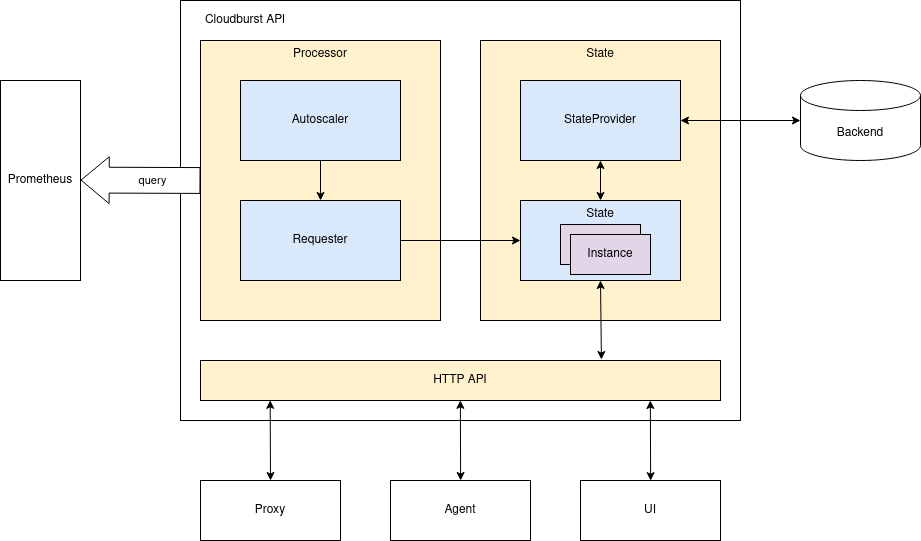
\includegraphics[width=1.0\linewidth,scale=1.0]{images/autoscaler.png}
	\caption{Hier muss was hin}
\end{figure}

\subsubsection{Configuration}
	
\subsubsection{Processor}
	
\subsubsection{Autoscaler}

\begin{figure}[h]
	\centering
	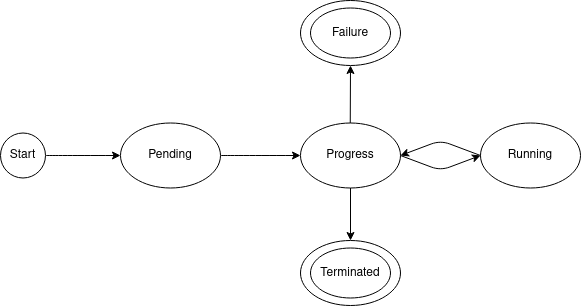
\includegraphics[width=0.8\linewidth,scale=0.8]{images/state.png}
	\caption{Hier muss was hin}
\end{figure}
	
\subsubsection{Requester}
	
\subsection{Agents}
	
\subsection{Proxy}

\subsection{Skalierungstechnik}

\section{Experimente}
	
	
\section{Ausblick}
	
% ---- Bibliography ----
%
% BibTeX users should specify bibliography style 'splncs04'.
% References will then be sorted and formatted in the correct style.
%
\newpage
\bibliographystyle{splncs04}
\bibliography{paper.bib}
%
\end{document}
